

 
\documentclass[12pt]{article}
 
\usepackage[margin=1in]{geometry} 
\usepackage{amsmath,amsthm,amssymb}
\usepackage{graphicx}
 
\begin{document}
 

 
\title{Resultados Tarea 4}
\author{Benjamin Leon\\
Metodos Computacionales tarea \# 4} 
\maketitle


\section{Ecuaciones diferenciales Ordinarias (ODE)}
\begin{centering}
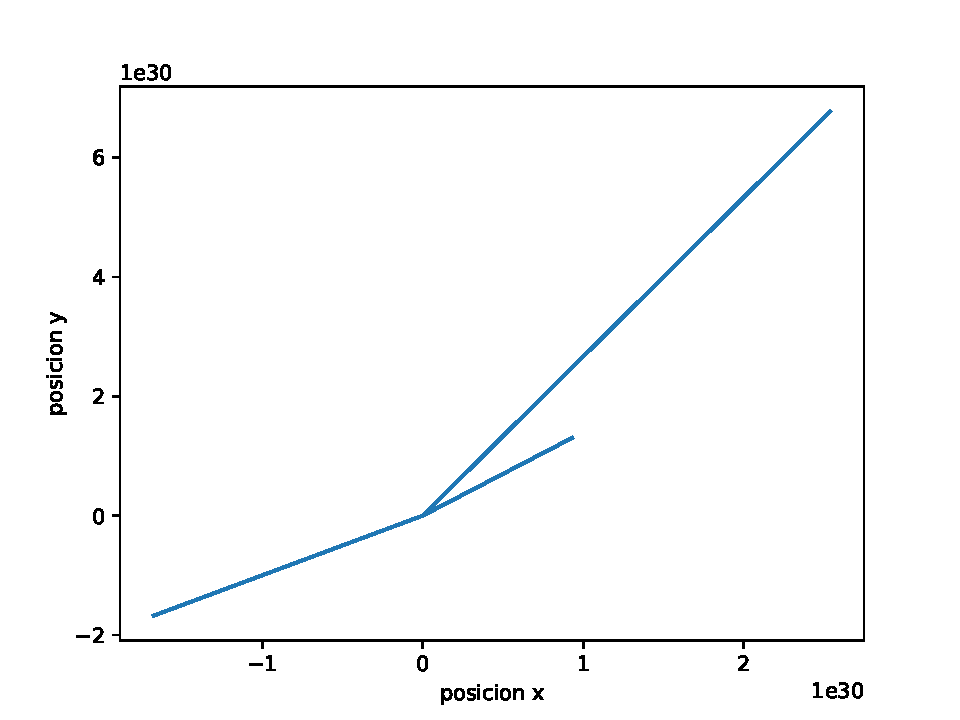
\includegraphics[width=0.75\textwidth]{grafsODE.pdf}

Deberia mostrar las diferentes trayectorias seg\'un el angulo de lanzamiento, pero por alg\'un error muestra lineas rectas

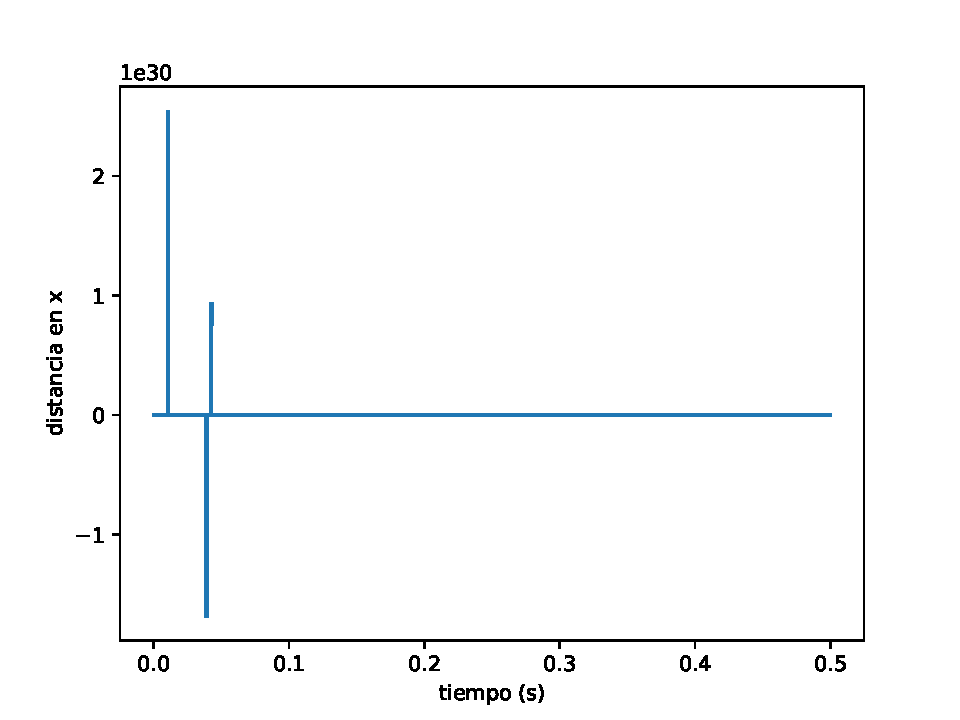
\includegraphics[width=0.75\textwidth]{grafsODE2.pdf}

Muestra la posicion en "x" con respecto al tiempo "t"

\includegraphics[width=0.75\textwidth]{10grados.pdf}

Ejemplo de lo que decimos en la secci\'on de comentarios de que la escala esconde alguna de las graficas aunque de todos modos se nota que los resultados no son correctos, esta grafica nos muestra que no en todos los casos la distancia diverge. Esta grafica nos muestra el procesamiento para un lanzamiento a 10 grados sobre el suelo.
\end{centering}


\section{Ecuaciones diferenciales Parciales(PDE)}

\begin{centering}

\subsection{Fronteras Fijas}
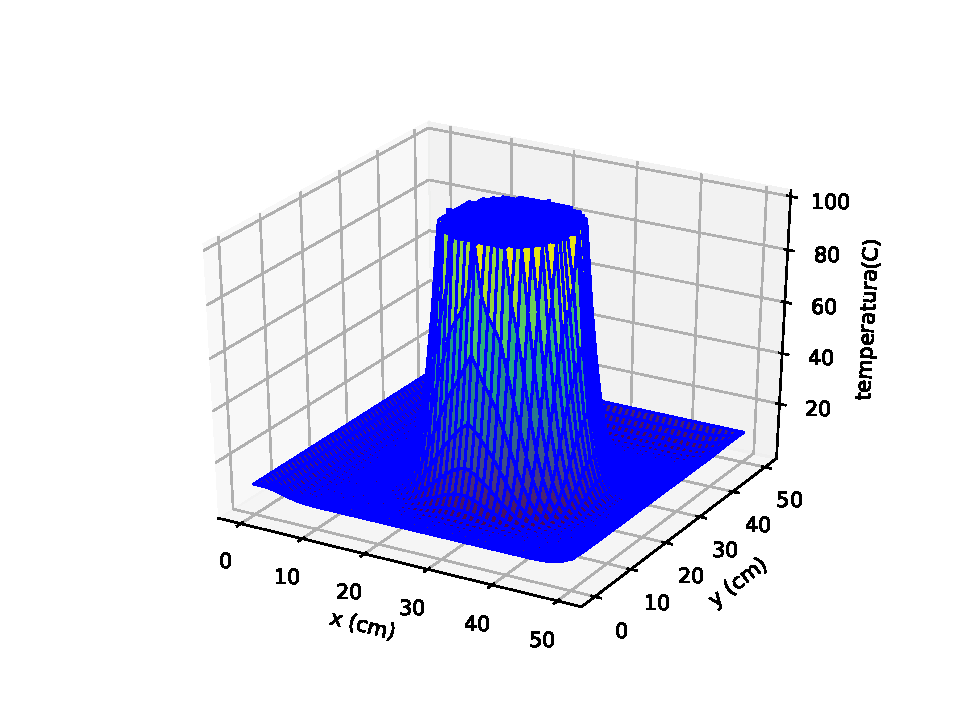
\includegraphics[width=0.75\textwidth]{3d2.pdf}
paso 10000
\\
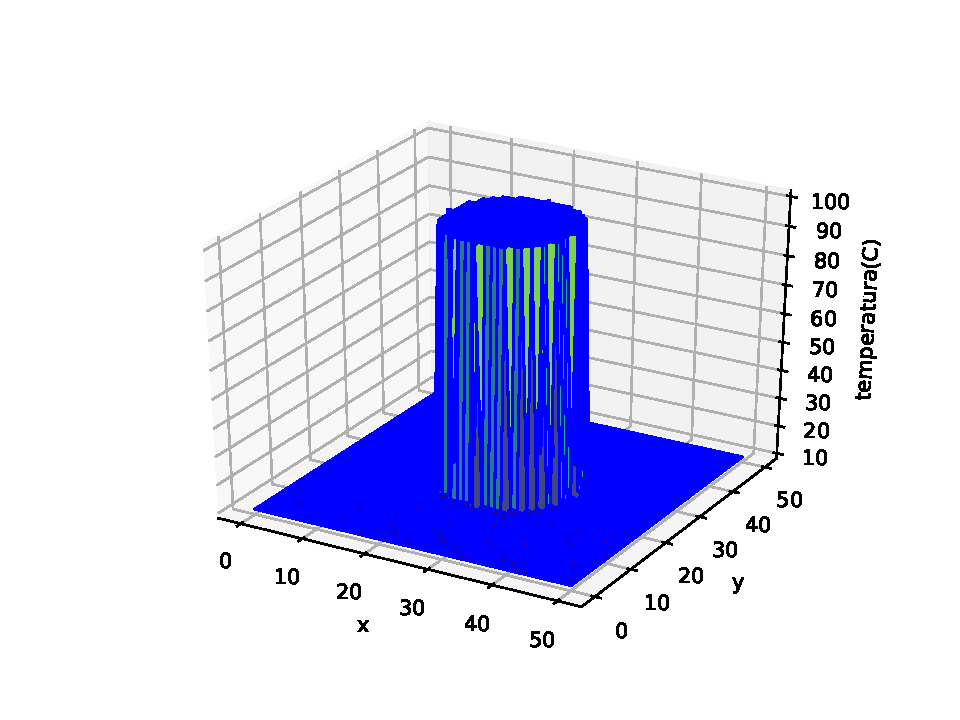
\includegraphics[width=0.75\textwidth]{3d3.pdf}
Paso 100
\\
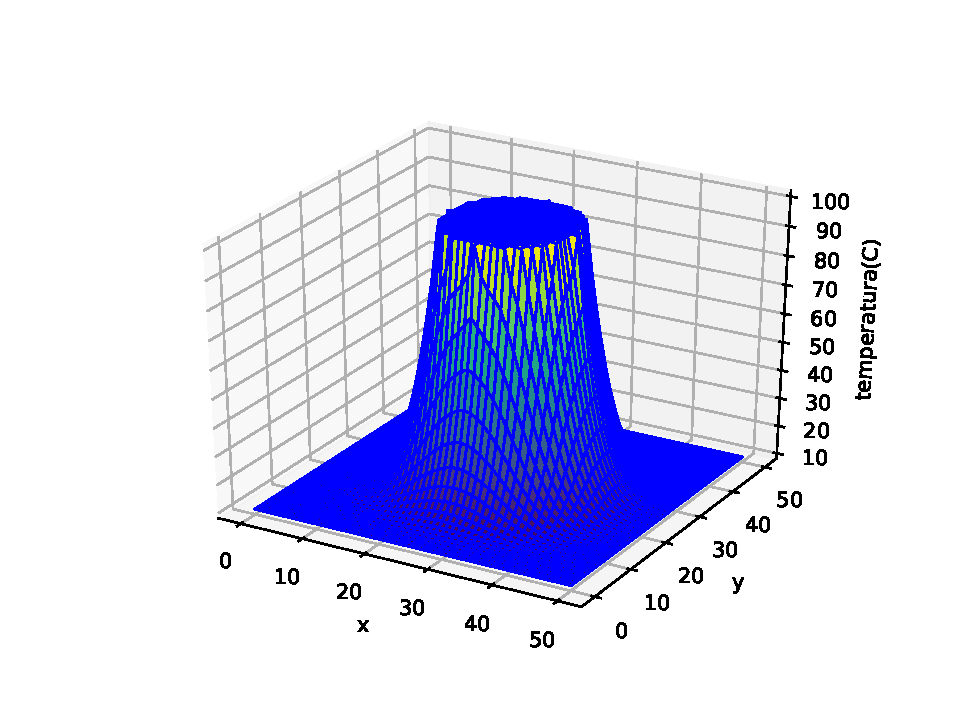
\includegraphics[width=0.75\textwidth]{3d4.pdf}
paso 1500
\subsection{Fronteras Abiertas}
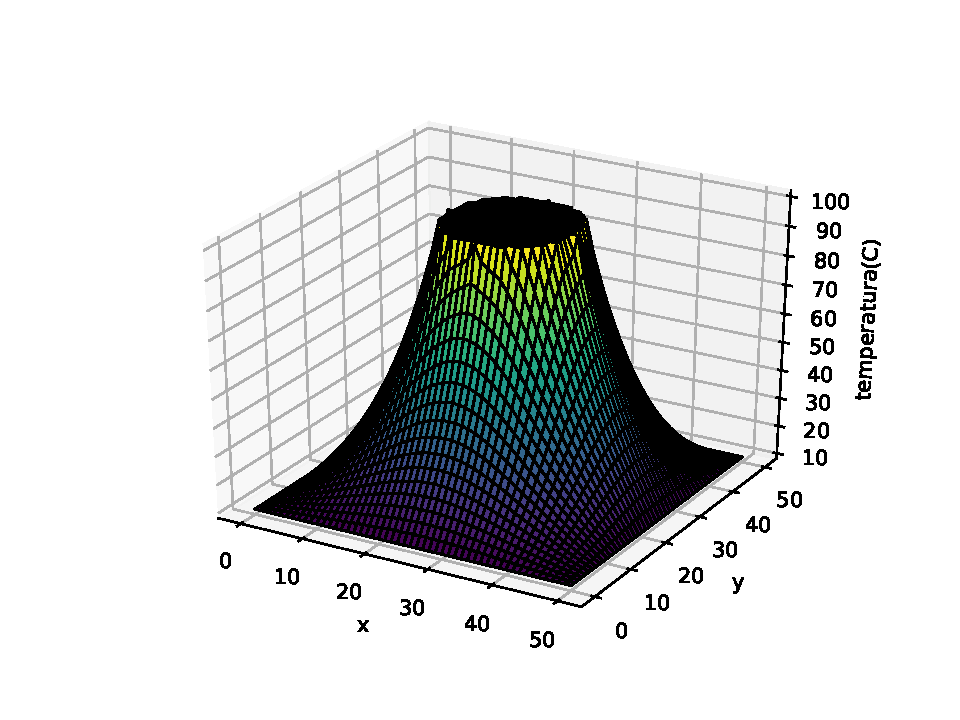
\includegraphics[width=0.75\textwidth]{3d5.pdf}
paso 10000
\\
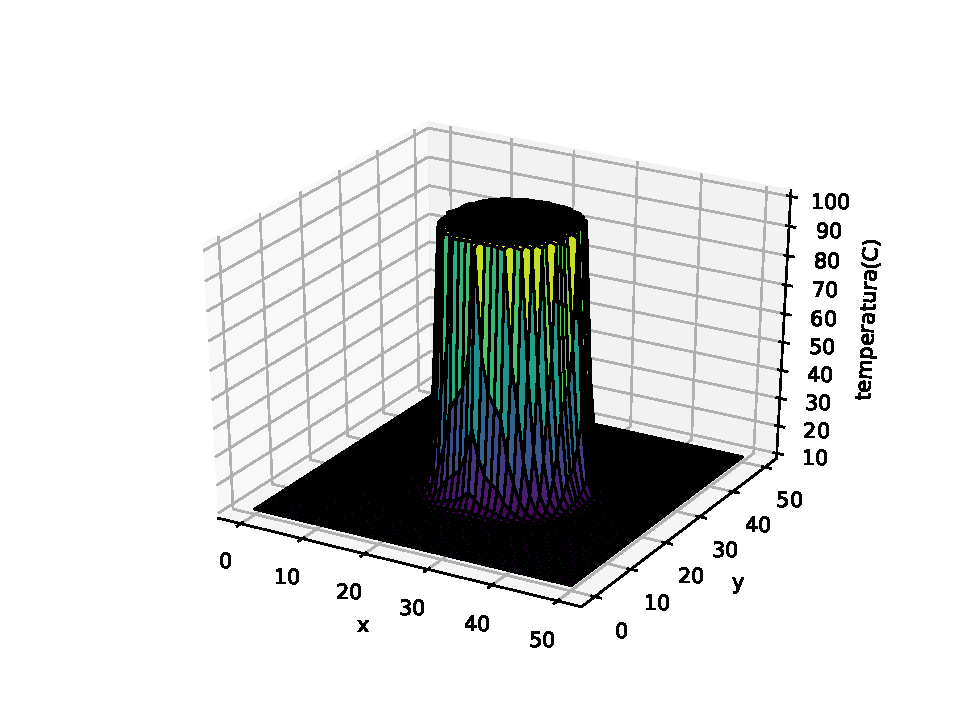
\includegraphics[width=0.75\textwidth]{3d6.pdf}
paso 100
\\
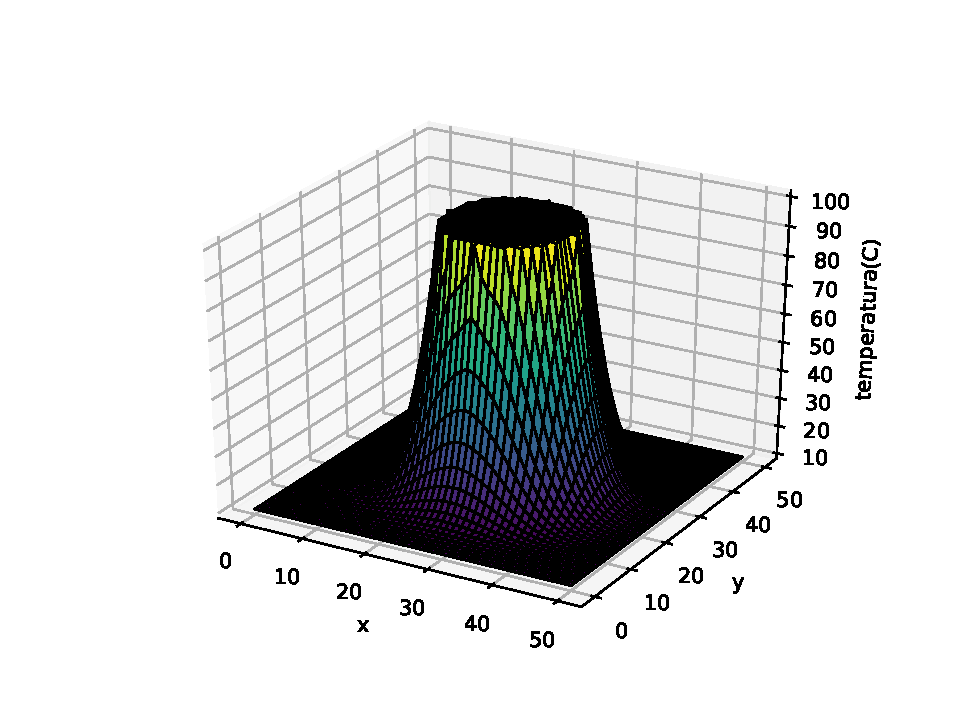
\includegraphics[width=0.75\textwidth]{3d7.pdf}
paso 1500
\subsection{Fronteras Periodicas}
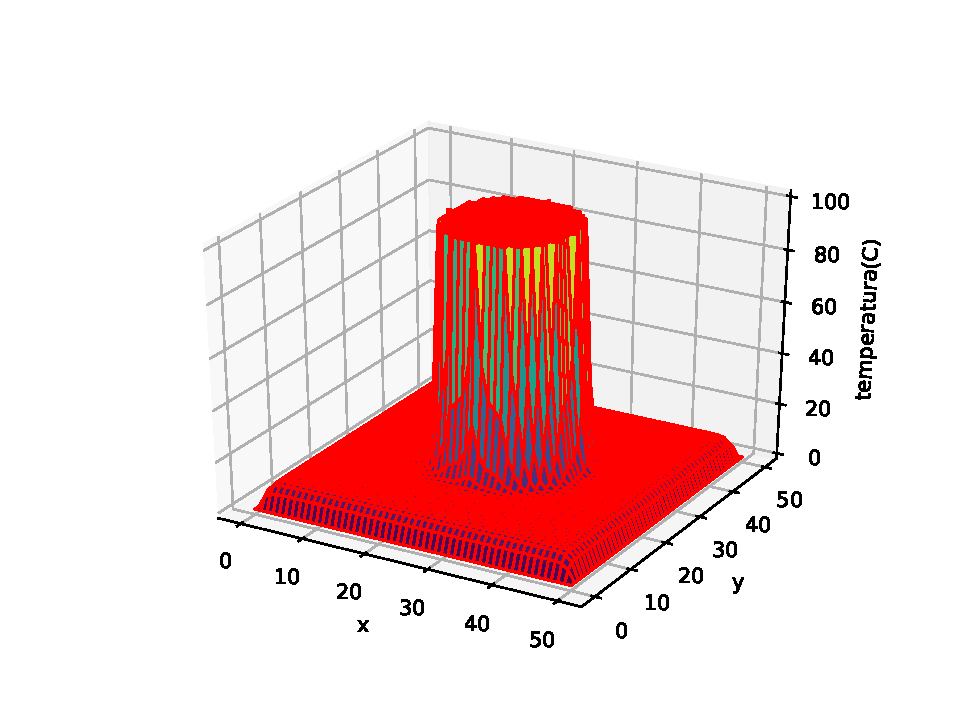
\includegraphics[width=0.75\textwidth]{3d8.pdf}
paso 10000
\\
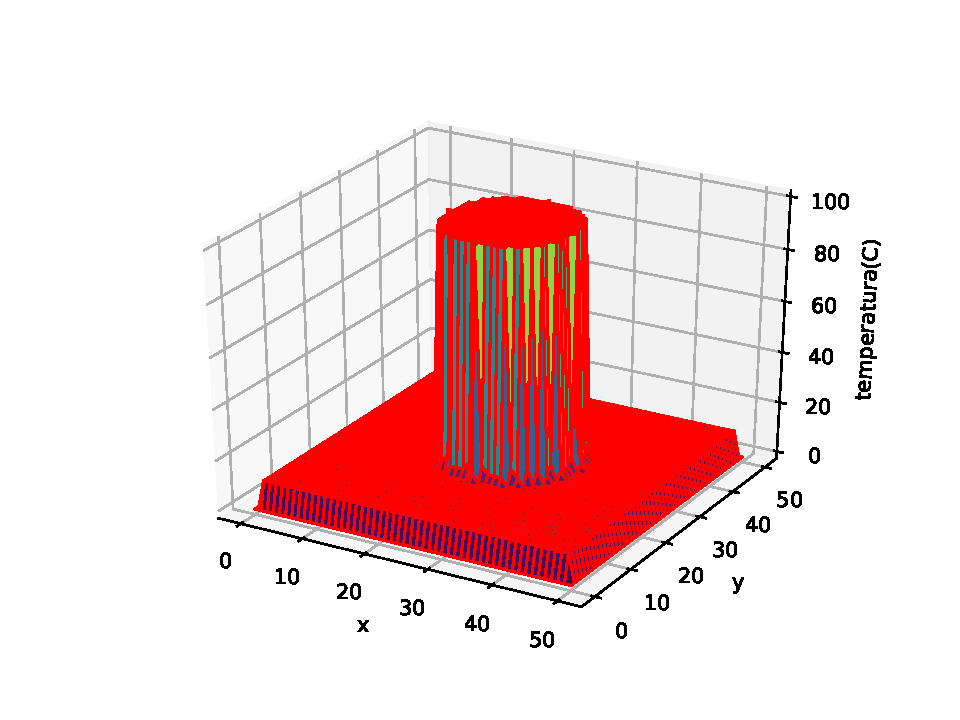
\includegraphics[width=0.75\textwidth]{3d9.pdf}
paso 100
\\
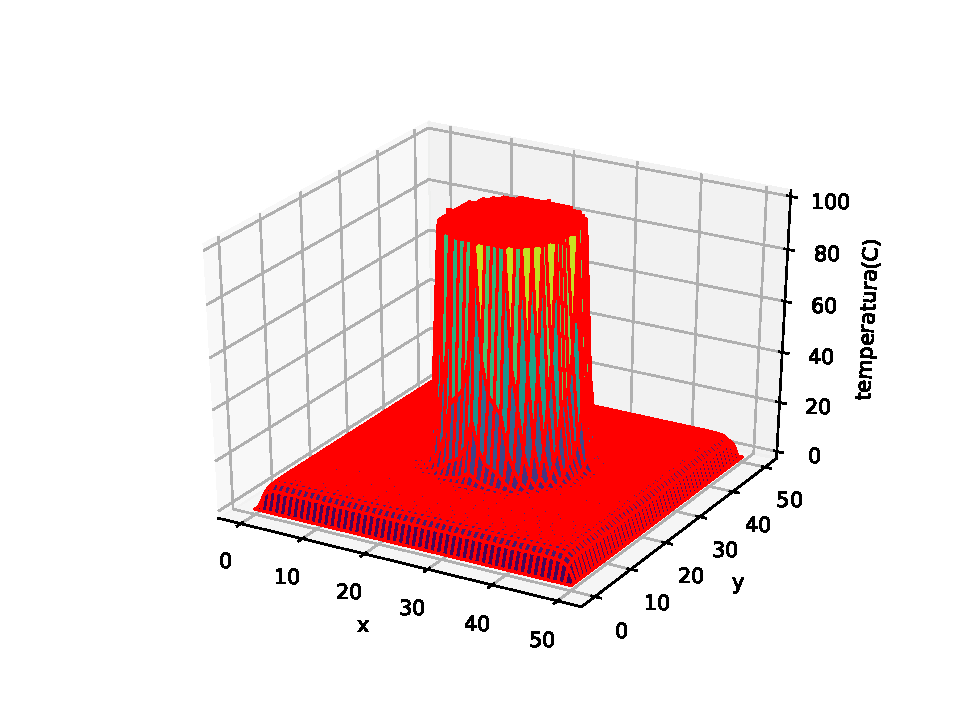
\includegraphics[width=0.75\textwidth]{3d10.pdf}
paso 1500


\end{centering}
\section{Comentarios}
El mayor problema encontrado fue en la parte de ODE donde no se pudo encontrar resultados validos para un tiro parabolico. Aunque si es problema de codigo no se pudo encontrar el origen del error aunque lo mas probable es que fuera en la implementaci\'on del metodo del "primer paso" o la implementaci\'on del metodo que genera el siguiente paso. En los resultados vemos que despues de pocos pasos (orden de 200) tanto las velocidades como los desplazamientos divergen a +- infinito. 
\\
Si observamos las graficas del punto de ODE por separado vemos que hay unas que no divergen pero son escondidas por la escala en de la grafica. Aunque no entiendo cual es la raz\'on de esto ya que el codigo parece estar correcto se ve en las dos graficas 
\\
En la parte de PDE se encontro un problema en encontrar los valores optimos para el numero de pasos y para el dt (cambio del tiempo) lo cual causa que despues de 10'000 iteraciones, el cambio desde las condiciones iniciales no sea muy grande. Tambien hubo complicaciones al correr el codigo completo desde el makefile ya que para hacer cada prueba, el programa se demora mas de 10 minutos en mi computador personal, probablemente por el numero de pasos utilizado. Este problema atraso el desarrollo de la actividad porque no se logro hacer multiples prubas variando los valores de pasos y de dt.
\\
Al final, las 3 graficas del paso 10'000 se ven muy parecidas, lo que nos dice que el estado de equilibrio es similar en los 3 casos. Para el caso de fronteras abiertas se utilizo un estado inicial donde los bordes estan a 10 grados pero para cada paso subsecuente no se reitera este valor entonces quedan libres.No fue muy claro que son las fronteras periodicas entonces se utilizo una funcion sinusoidal que varia entre 25 y -25 con un periodo de 200 pasos.
\\
En conclusi\'on podemos afirmar que fue exitoso el trabajo hecho ya que todo quedo completo y hay resultados claros que nos demuestran como los metodos numericos asociados con la programaci\'on y la computaci\'on nos pueden ser muy utiles para estudiar sistemas complejos. Se pudo haber complejisado el sistema utilizando matrizes de 5000 por 5000 para obtener resultados aun mas precisos pero esto solo hubiera alentado el proceso y tendriamos resultados muy similares.


\end{document}
